\documentclass[a4paper,oneside,twocolumn,notitlepage,dvipdfmx]{jsarticle}
\usepackage[utf8]{inputenc}
\usepackage{amsmath}
\usepackage{amsfonts}
\usepackage{amssymb}
\usepackage{makeidx}
\usepackage{graphicx}
\usepackage{color}
\usepackage{sample}
\usepackage{url}
\usepackage{listings,jlisting}
\setlength\abovecaptionskip{1pt}
\def\baselinestretch{0.3}


\lstset{
  basicstyle={\ttfamily},
  identifierstyle={\small},
  commentstyle={\smallitshape},
  keywordstyle={\small\bfseries},
  ndkeywordstyle={\small},
  stringstyle={\small\ttfamily},
  frame={tb},
  breaklines=true,
  columns=[l]{fullflexible},
  numbers=left,
  xrightmargin=0zw,
  xleftmargin=3zw,
  numberstyle={\scriptsize},
  stepnumber=1,
  numbersep=1zw,
  lineskip=-0.5ex
}

% 以下内容

\student{谷澤 悠太}
\date{令和5年11月8日}
\prof{滝沢 寛之}
\title{中間報告}
%\author{Maohua Zhu, Tao Zhang, Zhenyu Gu, Yuan Xie}
%\journal{MICRO-52, October 12-16, 2019, Columbus, OH, USA}
\nendo{令和5年度}

\begin{document}
\maketitle
\section{背景}
HPCは現在,機械学習や数値シュミレーション,統計解析など様々な科学分野で地擁されている.そのため,HPCを専門としない科学者がHPCを利用する事例が多く存在する.しかしながら,このような事例の場合,HPCを使いこなすための学習による時間や労力のコストが大きく,本来の研究に費やすコストが減少してしまうため問題となっている.\par
このような問題に対して,米国オハイオ・スーパーコンピューティングセンターはWebポータル上からHPCシステムを簡易に利用可能とする『Open OnDemand』(OOD)というソフトウェアを開発した.開発当時のOODはSLURM,Torque,PBS Pro,LSFなどのスケジューラに対応していた.しかしながら,対応していないスケジューラも多く,使える環境が限定されていたといえる.\par
そこで先行事例として,OODをFujitsu\_TCS(スーパーコンピュータ富岳で運用されているジョブスケジューラ)へ対応させたことによる『富岳』でのOOD利用という事例がある.\cite{meinronbun}これにより,『富岳』の利用者はHPCシステムの視覚的理解が容易になったり,利用難易度が低下したりといったメリットを得ることができた.\par

\section{目的}
本研究では東北大学で用いられているスーパーコンピュータ『AOBA』に着目して『AOBAへのOpen Ondemand導入によるスパコン利用者支援』を考える.前述の通り,OODには『AOBA』に用いられているジョブスケジューラNQSV(Network Queuing System V)に対応するためのアダプタが存在しない.そのため,AOBA用のアダプタを実装することでAOBA利用者の支援を目的とする.\par

\section{実装手順}
具体的な実装について,大きく4つの手順に分けて紹介する.\par
まず, 1つ目の手順としてSLURMスケジューラを試用しているsendaiサーバでOODの動作確認を行う.この手順でOODがどのようなものか理解したり,システムの設計について調査し,具体的な実装手順を見据える.\par
2つ目の手順として,SLURM用に書かれたアダプタファイルを自分で書き換えることでOODにその変更内容が反映されるかどうかを確認する.\par
3つ目の手順として,他のスケジューラのアダプタを参考にしてNQSVのアダプタを作成する.このとき,NQSVと親和性の高いPBS Proや動作確認で試用したSLURM,アダプタ作成例が紹介されているFujitsu\_TCSのアダプタなどを参考にする.\par
最後の手順として,手順2や手順3の過程からアダプタの構造理解やその汎用性などの検討を行う.アダプタやスケジューラの理解を深めることで,様々なスケジューラに対応できる汎用性の高いアダプタについて考察したい.

\section{進捗}

\subsection{OOD導入手順}
現在の進捗として,手順1で示したSLURM環境でのOODの動作確認が終了している.以降に動作確認で用いた動作環境と導入手順を示す.\par
OODの導入は大きく4つのステップで手順が実行さてていく.1ステップ目が環境構築,2ステップ目が必要なソフトウェアのインストール,3つ目がOODに必要な認証システムの構築である.\par

\subsubsection{環境構築}
まず,ステップ1の動作環境についてである.SLURMスケジューラを用いたsendaiサーバで実行していてOSはUbuntu22.04.1 LTSを用いてsudo権のある一般ユーザーで実行している.\par

\subsubsection{パッケージインストール}
続いてOODのインストールに際して,必要なパッケージのインストールを行う.Apach HTTP Server 2.4とRuby 2.7,Node.js 14が用いられるためインストールを行う.その後,公式のドキュメントに従ってリポジトリを追加し,OODのインストールを行う.その後,SystemctlコマンドによりApacheを起動する.UbuntuではApacheによるデフォルトページが表示されてしまうため,/etc/ood/config/ood\_portal.yml のservernameをデフォルトの状態から設定したいドメインに変更する必要がある.これにより,設定ドメインにアクセスするとOODの認証システム構築待機画面が表示され,認証システムの構築を指示される.\par

\begin{figure}[h]
  \centering
  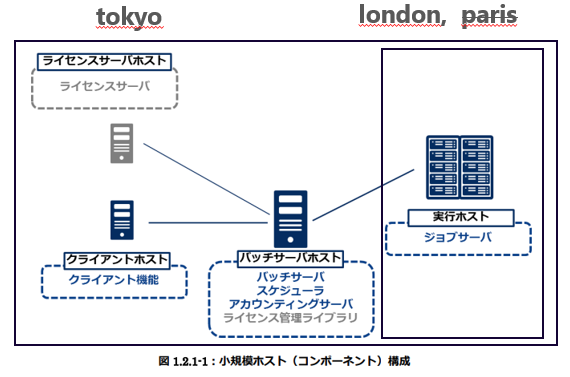
\includegraphics[width=75mm]{./fig/globalseminar_20231109/fig_1.png}
  \caption{認証システムの設計}
  \label{fig_1}
\end{figure}

\subsubsection{認証システム}
指示に従い,認証の設定を行う.今回はデフォルトで推奨されている「DexとのOpenIDコネクト」という方法を用いて認証を行う.これに付随してLDAPサーバが必要となるため,必要に応じてLDAPサーバを構築する必要がある.ここで,OpenIDコネクトとはユーザ認証用のプロトコルを指し,DexとはOpenIDコネクト認証のプロバイダー,LDAPサーバとは認証に必要なユーザ情報を管理するディレクトリサーバである.また,今回の動作環境では研究室内のアカウント情報を管理しているActiveDirectiory(AD)を用いる.ADはWindows用のディレクトリサーバであり,中身はLDAPサーバと同じであるため,問題なく接続できる.\par
ここで,認証システムの設計を図\ref{fig_1}に示す.このように,今回はOODとDexサーバが同一のマシンで動作し,DexにtivelaサーバのADを接続して用いる.\par
認証システムの構築手順として,まずOnDemand-dexのパッケージのインストールを行い、続いてOnDemand-dexとADの接続,その後OnDemand-dexの起動を行う.OnDemand-dexとADの接続について,接続ファイルであるood\_portal.ymlを書き換える必要があるため,以降に手順の詳細を示す.\par
ADとの接続設定は/etc/ood/config/ood\_portal.ymlに記載されている.接続設定が書かれたファイル内のdexキー以下を図\ref{fig_2}に示す.hostキーはADのドメインとポート番号を示し,今回はSSLを用いたLDAPで接続するので636番を用いる.insecureSkipVerifyは証明書の検証の有無を示し,今回はスキップする.bindDNとbindPWはADの管理者アカウントの識別名とパスワードを示す.また,usersearch,groupsearchはそれぞれユーザ探索グループ探索に用いる情報を示していて,baseDNはそれぞれの探索の開始位置の識別名である.ADのディレクトリは木構造になっていて,すべてのユーザがDN(識別名)で認識される.参考として図\ref{fig_3}にツリー構成の例を示す.\par
また,Dexの背後にSQLが動いているため/etc/ood/dex/config.yamlで記載されているstorageキー配下を設定する必要がある.デフォルトで推奨されているsqliteのインストールを行った後,図\ref{fig_4}に示すようにstorageのtypeの変更とconfigのfileのパスを正しいものに修正する.\par
以上の作業により認証システムが機能し,ADに登録してあるusernameとpasswordを用いてOODにログインすることが可能となった.\par

\begin{figure}[h]
  \centering
  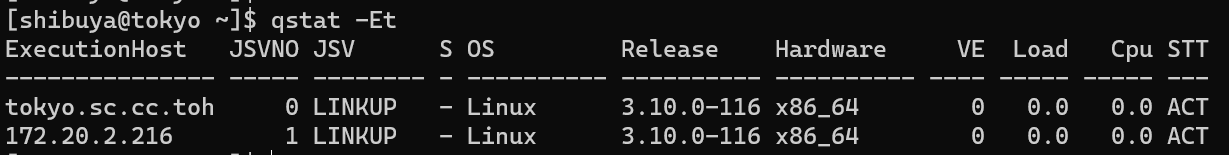
\includegraphics[width=75mm]{./fig/globalseminar_20231109/fig_2.png}
  \caption{ood\_portal.yml}
  \label{fig_2}
\end{figure}

\begin{figure}[h]
  \centering
  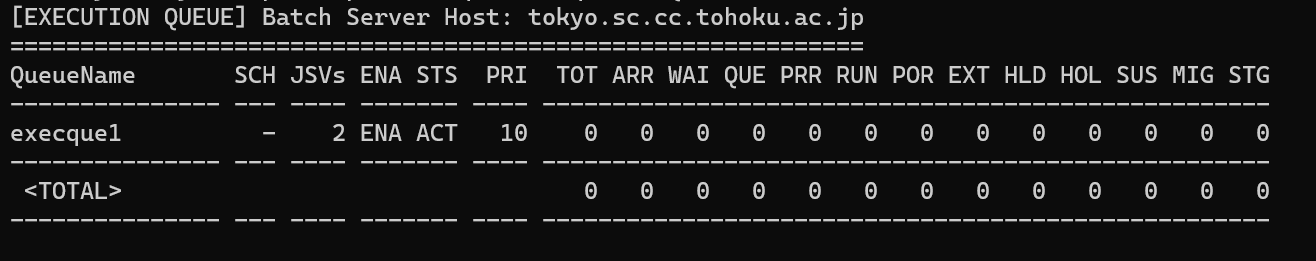
\includegraphics[width=75mm]{./fig/globalseminar_20231109/fig_3.png}
  \caption{ADの構造}
  \label{fig_3}
\end{figure}

\begin{figure}[h]
  \centering
  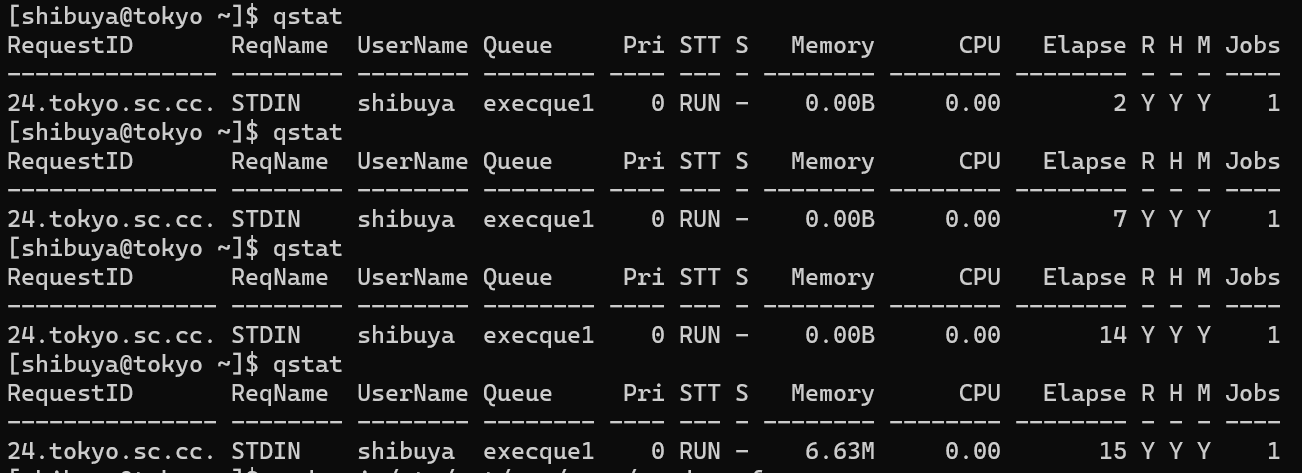
\includegraphics[width=75mm]{./fig/globalseminar_20231109/fig_4.png}
  \caption{SQLの設定}
  \label{fig_4}
\end{figure}

\subsection{クラスタ構築}
最後のステップとしてクラスタ構成の設定を行う.クラスタの構成は/etc/ood/config/cluster.d/sendai.ymlを作成し,図\ref{fig_5}のように記述する.titleはクラスタ名,hostはログインするサーバのドメインを表し,adaperは試用するジョブスケジューラ,binとconfは使用するスケジューラのbinディレクトリとconfigファイルのパスを表す.この設定によりOODがsendaiクラスタを認識し,各アプリケーションが使用できるようになる.\par

\begin{figure}[h]
  \centering
  \includegraphics[width=75mm]{./fig/globalseminar_20231109/fig_5.png}
  \caption{クラスタ構成}
  \label{fig_5}
\end{figure}

\subsection{Job Composer}
OODの動作確認をするために設定したクラスタにジョブを投入する「Job Composer」というアプリケーションを使ってジョブを投入してみる.図\ref{fig_6}が「Job Composer」のジョブ選択画面である.New JobからFrom Specified Pathを選択して,実行ファイルのパスと名前,実行クラスタを選択.その後,登録した実行ジョブを選択してSubmitすることでジョブの投入を行うことができる.実際に投入されたジョブの状態は「Active Job」から確認することが可能であり,実行されたジョブのステータスや実行時間などを確認することができた.\par

\begin{figure}[h]
  \centering
  \includegraphics[width=75mm]{./fig/globalseminar_20231109/fig_6.png}
  \caption{Job Composer}
  \label{fig_6}
\end{figure}


\section{今後の予定}
短期目標として,\par
・各スケジューラのアダプタのコードの読み込みと理解\par
・SLURMアダプタの書き換えと書き換えたアダプタの動作確認\par
中長期目標として,\par
・NQSVのアダプタを作成する際のテスト環境準備
・NQSVのアダプタの作成
を考えている.\par



\bibliographystyle{junsrt}
\bibliography{refer}


\end{document}